% Format teze zasnovan je na paketu memoir
% http://tug.ctan.org/macros/latex/contrib/memoir/memman.pdf ili
% http://texdoc.net/texmf-dist/doc/latex/memoir/memman.pdf
% 
% Prilikom zadavanja klase memoir, navedenim opcijama se podešava 
% veličina slova (12pt) i jednostrano štampanje (oneside).
% Ove parametre možete menjati samo ako pravite nezvanične verzije
% mastera za privatnu upotrebu (na primer, u b5 varijanti ima smisla 
% smanjiti 
\documentclass[12pt,oneside]{memoir}

% Paket koji definiše sve specifičnosti mastera Matematičkog fakulteta
\usepackage[latinica]{matfmaster}
\usepackage{graphicx}

\definecolor{codegray}{gray}{0.9}
\newcommand{\code}[1]{\colorbox{codegray}{\texttt{\scalebox{0.9}{#1}}}}%
% Podrazumevano pismo je ćirilica.
%   Ako koristite pdflatex, a ne xetex, sav latinički tekst na srpskom jeziku
%   treba biti okružen sa \lat{...} ili \begin{latinica}...\end{latinica}.
%
% Opicija [latinica]:
%   ako želite da pišete latiniciom, dodajte opciju "latinica" tj.
%   prethodni paket uključite pomoću: \usepackage[latinica]{matfmaster}.
%   Ako koristite pdflatex, a ne xetex, sav ćirilički tekst treba biti
%   okružen sa \cir{...} ili \begin{cirilica}...\end{cirilica}.
%
% Opcija [biblatex]:
%   ako želite da koristite reference na više jezika i umesto paketa
%   bibtex da koristite BibLaTeX/Biber, dodajte opciju "biblatex" tj.
%   prethodni paket uključite pomoću: \usepackage[biblatex]{matfmaster}
%
% Opcija [b5paper]:
%   ako želite da napravite verziju teze u manjem (b5) formatu, navedite
%   opciju "b5paper", tj. prethodni paket uključite pomoću: 
%   \usepackage[b5paper]{matfmaster}. Tada ima smisla razmisliti o promeni
%   veličine slova (izmenom opcije 12pt na 11pt u \documentclass{memoir}).
%
% Naravno, opcije je moguće kombinovati.
% Npr. \usepackage[b5paper,biblatex]{matfmaster}

% Pomoćni paket koji generiše nasumičan tekst u kojem se javljaju sva slova
% azbuke (nema potrebe koristiti ovo u pravim disertacijama)
\usepackage{pangrami}

% Paket koji obezbeđuje ispravni prikaz ćiriličkih italik slova kada
% se koristi pdflatex. Zakomentarisati ako na sistemu koji koristite ovaj
% paket nije dostupan ili ako ne radi ispravno.
\usepackage{cmsrb}
\usepackage[font={small}]{caption}
% Ostali paketi koji se koriste u dokumentu
\usepackage{listings} % listing programskog koda
\usepackage{color} %use color
\definecolor{mygreen}{rgb}{0,0.6,0}
\definecolor{mygray}{rgb}{0.5,0.5,0.5}
\definecolor{mymauve}{rgb}{0.58,0,0.82}
\definecolor{lightgray}{rgb}{.9,.9,.9}

% %Customize a bit the look
% \lstset{ %
% backgroundcolor=\color{white}, % choose the background color; you must add \usepackage{color} or \usepackage{xcolor}
% basicstyle=\footnotesize, % the size of the fonts that are used for the code
% breakatwhitespace=false, % sets if automatic breaks should only happen at whitespace
% breaklines=true, % sets automatic line breaking
% captionpos=b, % sets the caption-position to bottom
% commentstyle=\color{mygreen}, % comment style
% deletekeywords={...}, % if you want to delete keywords from the given language
% escapeinside={\%*}{*)}, % if you want to add LaTeX within your code
% extendedchars=true, % lets you use non-ASCII characters; for 8-bits encodings only, does not work with UTF-8
% frame=false, % adds a frame around the code
% keepspaces=true, % keeps spaces in text, useful for keeping indentation of code (possibly needs columns=flexible)
% keywordstyle=\color{blue}, % keyword style
% % language=Octave, % the language of the code
% morekeywords={*,...}, % if you want to add more keywords to the set
% numbers=left, % where to put the line-numbers; possible values are (none, left, right)
% numbersep=5pt, % how far the line-numbers are from the code
% numberstyle=\tiny\color{mygray}, % the style that is used for the line-numbers
% rulecolor=\color{black}, % if not set, the frame-color may be changed on line-breaks within not-black text (e.g. comments (green here))
% showspaces=false, % show spaces everywhere adding particular underscores; it overrides 'showstringspaces'
% showstringspaces=false, % underline spaces within strings only
% showtabs=false, % show tabs within strings adding particular underscores
% stepnumber=1, % the step between two line-numbers. If it's 1, each line will be numbered
% stringstyle=\color{mymauve}, % string literal style
% tabsize=2, % sets default tabsize to 2 spaces
% title=\lstname % show the filename of files included with \lstinputlisting; also try caption instead of title
% }
%END of listing package%
 
\definecolor{darkgray}{rgb}{.4,.4,.4}
\definecolor{purple}{rgb}{0.65, 0.12, 0.82}
%define Javascript language
\lstdefinelanguage{JavaScript}{
keywords={typeof, class, extends, export, new, true, false, catch, function, return, null, catch, switch, var, if, in, while, do, else, case, break},
keywordstyle=\color{blue}\bfseries,
ndkeywords={export, boolean, throw, implements, import, from, this},
ndkeywordstyle=\color{red}\bfseries,
identifierstyle=\color{black},
sensitive=false,
comment=[l]{//},
morecomment=[s]{/*}{*/},
commentstyle=\color{purple}\ttfamily,
stringstyle=\color{mygreen}\ttfamily,
moredelim=[s][\color{black}]{\$\{}{\}}, % same as morestring in this case
morestring=[d]{'},
morestring=[d]{`},
morestring=[d]{"},
}

\lstdefinelanguage{html}{
keywords={body, div, script},
keywordstyle=\color{blue}\bfseries,
ndkeywords={class, export, boolean, throw, implements, import, this},
ndkeywordstyle=\color{darkgray}\bfseries,
identifierstyle=\color{black},
sensitive=false,
comment=[l]{//},
morecomment=[s]{/*}{*/},
commentstyle=\color{purple}\ttfamily,
stringstyle=\color{mygreen}\ttfamily,
morestring=[b]',
morestring=[b]"
}

\lstset{
language=JavaScript,
extendedchars=true,
basicstyle=\footnotesize\ttfamily,
backgroundcolor=\color{white},
showstringspaces=false,
showspaces=false,
numbers=none,
numberstyle=\footnotesize,
numbersep=9pt,
tabsize=2,
breaklines=true,
showtabs=false,
captionpos=b,
}

\lstdefinelanguage{shell}{
keywords={\$, \> },
keywordstyle=\color{red}\bfseries,
ndkeywords={class, export, boolean, throw, implements, import, this},
ndkeywordstyle=\color{darkgray}\bfseries,
identifierstyle=\color{black},
sensitive=false,
morecomment=[s]{/*}{*/},
commentstyle=\color{purple}\ttfamily,
stringstyle=\color{mygreen}\ttfamily,
morestring=[b]',
morestring=[b]`,
morestring=[b]"
}
\lstset{
language=shell,
extendedchars=true,
basicstyle=\footnotesize\ttfamily,
backgroundcolor=\color{lightgray},
frame=single,
showstringspaces=false,
showspaces=false,
numbers=none,
numberstyle=\footnotesize,
numbersep=9pt,
tabsize=2,
breaklines=true,
showtabs=false,
captionpos=b
}
\lstdefinestyle{htmlStyle} {language=html,backgroundcolor=\color{white},frame=single}
\lstdefinestyle{jsStyle} {language=JavaScript,backgroundcolor=\color{white},frame=single, numbers=left, numberstyle=\tiny, }
\lstdefinestyle{shellStyle} {language=shell,backgroundcolor=\color{lightgray},frame=single}
\newcounter{shellRef}[chapter]

\newcommand{\shellcmd}[2]{\\\\\texttt{\footnotesize\$ #1 \null\hfill (\refstepcounter{shellRef}{\theshellRef})\label{#2} }\\\\}
\renewcommand{\theshellRef}{\thechapter.\number\numexpr\value{shellRef}\relax}

\renewcommand\lstlistingname{Isečak koda}
% Datoteka sa literaturom u BibTex tj. BibLaTeX/Biber formatu
\bib{matfmaster-primer}

% Ime kandidata na srpskom jeziku (u odabranom pismu)
\autor{Aleksandar Milosavljević}
% Naslov teze na srpskom jeziku (u odabranom pismu)
\naslov{Razvoj "Pure" okruženja za razvoj veb interfejsa}
% Godina u kojoj je teza predana komisiji
\godina{2021}
% Ime i afilijacija mentora (u odabranom pismu)
\mentor{dr Saša \textsc{Malkov}, vanredni profesor\\ Univerzitet u Beogradu, Matematički fakultet}
% Ime i afilijacija prvog člana komisije (u odabranom pismu)
\komisijaA{dr Aleksandar \textsc{Kartelj}, docent\\ Univerzitet u Beogradu, Matematički fakultet}
% Ime i afilijacija drugog člana komisije (u odabranom pismu)
\komisijaB{dr Ivan \textsc{Čukić}, docent\\ Univerzitet u Beogradu, Matematički fakultet}
% Ime i afilijacija trećeg člana komisije (opciono)
% \komisijaC{}
% Ime i afilijacija četvrtog člana komisije (opciono)
% \komisijaD{}
% Datum odbrane (obrisati ili iskomentarisati narednu liniju ako datum odbrane nije poznat)
\datumodbrane{15. јануар 2016.}

% Apstrakt na srpskom jeziku (u odabranom pismu)
\apstr{%
Rezime placeholder
}

% Ključne reči na srpskom jeziku (u odabranom pismu)
\kljucnereci{veb, internet, interfejs, html, css, javaskript, razvojno okruženje}

\begin{document}
% ==============================================================================
% Uvodni deo teze
\frontmatter
% ==============================================================================
% Naslovna strana
\naslovna
% Strana sa podacima o mentoru i članovima komisije
\komisija
% Strana sa posvetom (u odabranom pismu)
\posveta{Svima osim LaTex-u}
% Strana sa podacima o disertaciji na srpskom jeziku
\apstrakt
% Sadržaj teze
\tableofcontents*

% ==============================================================================
% Glavni deo teze
\mainmatter
% ==============================================================================

% ------------------------------------------------------------------------------
\chapter{Uvod}
Poboljšanje infrstrukture Internet mreže, to jest, povećanjem brzine i stabilnosti internet komunikacije,
naša interakcija sa računarima danas izgleda značajno drugačije nego pre 20 godina. Umesto stonih računara sa velikim kućištima i glasnim rashladnim sistemima,
današnji najrasprostranjeniji računari nam staju u džep. Koristimo ih kako bi komunicirali sa bližnjima i bili u toku sa svetskim dešavanjima.

Iako današnji mini računar koji gotovo svi nosimo u džepu ima više procesorske moći nego računar koji je korišćen tokom Appolo misije(ref), 
danas te lične računare ne koristimo za teška izračunavanja i komplikovane procedure. Koristimo ih najčešće kao terminale kako bismo pristupili internet resursima,
to jest, podacima koji se nalaze na velikim centralizovanim računarskim sistemima. Veb interfejs je tako postao glavni način naše interakcije sa računarom i internetom.

Posledica toga je značajna promena fokusa u svetu razvoja aplikativnog softvera. Ukoliko pogledamo rezultat upitnika kompanije "Stack Overflow" (ref)({\url{https://insights.stackoverflow.com/survey/2020#technology-programming-scripting-and-markup-languages-professional-developers}}) o najkorišćenijim programerskim alatima, videćemo da prva dva mesta na listi
zauzimaju upravo veb tehnologije (Na prvom mestu je JavaScript sa 69.7\%, dok je na drugom HTML/CSS sa 62.4\%).

Kako potreba za novim softverom daleko prevazilazi mogućnost softverskih inženjera da taj softver isporuče, biblioteke i okruženja koja pomažu pri razvoju softvera postali su veoma važan deo inženjerskog alata.
U domenu razvoja veb aplikacija, na tržištu se izdvajaju tri razvojna okruženja. Ova tri razvojna okruženja najviše se međusobno razlikuju po pristupu u promeni stanja aplikacije i razumevanju
toga šta je centralni deo dizajna (u funkcionalnom smislu) jedne veb aplikacije.

Kada posmatramo ova popularna razvojna okruženja, uočavamo dva bitno različita pristupa u arhitekturi:
\begin{enumerate}
  \item {\emph{Model-Pogled-Kontroler}} šablon u kom aplikacija predstavlja skup povezanih komponenti organizovanih u hijerarhisku strukturu, kojima je pridruženo stanje i ponašanje
  \item Flux šablon u kom se aplikacija posmatra kao mašina stanja čija je vizuelna reprezentacija samo rezultat trenutnog stanja.
\end{enumerate}

Prvi pristup je prisutan u okruženju Angular, drugi je dominantan u biblioteci React, dok Vue.js zastupa dizajn koji predstavlja kompromis izmеđu ova dva pristupa.

Kroz ovaj rad ispratićemo razvoj jednog modernog razvojnog okruženja za izradu SPA veb aplikacija.


% ------------------------------------------------------------------------------
\chapter{Arhitekture SPA aplikacija}
\section{Model-Pogled-Kontroler šablon}

\section{Flux šablon}
% ------------------------------------------------------------------------------
Razrada placeholder
% ------------------------------------------------------------------------------
\chapter{Problemi sa popularnim okruženjima}
\section{Upravljanje stanjem}
\section{Razdvajanje odgovornosti}
% ------------------------------------------------------------------------------
\chapter{Okruženje Pure}
Kako bismo se upoznali detaljnije sa novim okruženjem, krenućemo od jednostavnog
primera, \emph{Hello World (eng. Zdravo Svete)} aplikacije. 
\section{Podešavanje radnog okruženja}
Okruženje \emph{Pure} može se preuzeti kroz \emph{npm}\footnote{Upravljač paketa za Node \emph{(eng. Node Package Manager)}} sistem.
To možemo uraditi na dva načina:
\begin{enumerate}
  \item Instaliranjem paketa \code{pure-framework} u već postojeći \emph{npm} modul.
  \item Pokretanjem skripte za pravljenje \code{hello-world} projekta, bez prethodnog instaliranja \emph{npm} paketa.
\end{enumerate}
Ukoliko već imamo svoj \emph{npm} modul u kom pišemo kod, možemo iskoristiti prvi način i instalirati \code{pure-framework} komdanom \ref{cmd:npm-install}:
\shellcmd{npm install pure-framework}{cmd:npm-install}
Ovde ćemo, jednostavnosti radi, koristiti drugi pristup u kojem krećemo sa praznim folderom, u kom ćemo pomoću \emph{npx} skripte napraviti početnu "Zdravo Svete" aplikaciju.
Potrebno je da se u \code{shell}-u pozicioniramo u prazan direktorijum i da odatle pokrenemo komandu \ref{cmd:npx}:
\shellcmd{npx pure-framework hello-world}{cmd:npx}
Ova komanda će napraviti novi direktorijum sa nazivom \code{hello-world} i u njega klonirati repozitorijum sa minimalnom \emph{Pure} aplikacijom. 
Ukoliko je skripta izvršena bez grešaka, direktorijum \code{hello-world} bi trebalo da sadrži fajlove prikazane na slici \ref{fig:hello-world-direktorijum}.

\begin{figure}[!ht]
  \centering
  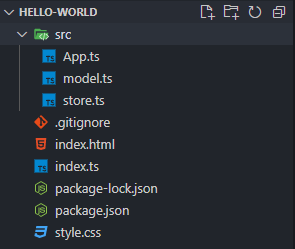
\includegraphics[width=0.5\textwidth]{slike/hello-world-direktorijum.PNG}
  \caption{Графикон}
  \label{fig:hello-world-direktorijum}
\end{figure}
Kako bismo pokrenuli našu aplikaciju, potrebno je da se pozicioniramo u novonapravljeni direktorijum i instaliramo neophodne \emph{npm} pakete,
izvršavanjem komande prikazane na isečku \ref{cmd:npm-install-hello-world}:
\shellcmd{cd hello-world \&\& npm install}{cmd:npm-install-hello-world}
Nakon što se ova komanda uspešno izvrši, možemo da pokrenemo našu aplikaciju komandom prikazanom na isečku \ref{cmd:npm-start}:
\shellcmd{npm run start}{cmd:npm-start}
Ukoliko pokretanje ove komande nije izbacilo grešku, konzola bi trebala da nas obavesti da je server za razvoj pokrenut i da možemo da mu pristupimo na url adresi \code{http://localhost:1234} (Isečak \ref{konzola:npmstart})\\
\renewcommand\lstlistingname{Izlaz konzole}
\begin{lstlisting}[style=shellStyle, caption={konzolna poruka nakon pokretanja aplikacije}, label=konzola:npmstart]
> pure-framework-hello-world-app@1.0.0 start
> parcel index.html

Server running at http://localhost:1234
Built in 27ms
\end{lstlisting}
\renewcommand\lstlistingname{Isečak koda}

Ukoliko u pretraživaču otvorimo url stranicu \code{http://localhost:1234}, trebalo bi da vidimo stranicu koja izgleda kao na slici \ref{fig:hello-world} 

\begin{figure}[!ht]
  \centering
  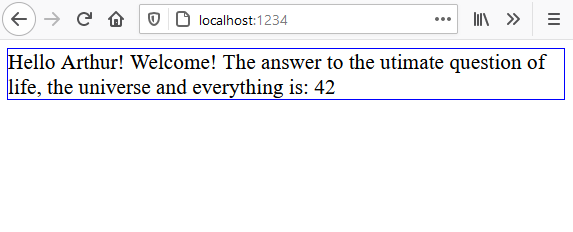
\includegraphics[width=0.8\textwidth]{slike/hello-world-strana.PNG}
  \caption{Hello World aplikacija, pokrenuta na lokalnom serveru.}
  \label{fig:hello-world}
\end{figure}

\section{Struktura aplikacije}
Pogledajmo sada sadržaj fajlova koje smo napravili u koraku \ref{cmd:npx}.
Primetićemo da fajlovi \code{index.html} i \code{index.ts} gotovo da ne sadrže nikakvu programsku logiku ili opis strukture DOM\footnote{ Document Object Model} drveta.
U narednim poglavljima upoznaćemo se detaljnije sa svrhom ovih fajlova, ali ćemo te detalje za sada preskočiti.

Fajl koji sadrži centralnu logiku naše aplikacije je \code{src/App.ts} (Isečak \ref{file:app.ts})
\pagebreak
\begin{lstlisting}[style=jsStyle, caption={Sadržaj fajla \code{App.ts}},label=file:app.ts]
import { Component, componentFactory, Store } from "pure-framework/core";
import { div, span } from "pure-framework/htmlElements";
import { AppModel } from "./model";

class AppComponent extends Component<AppModel> {
  template() {
    return div({ class: 'app-root'}, [
      span(`Hello ${this.state.name}! Welcome! `),
      span(`The answer to the utimate question of life, the universe and everything is: ${this.state.answer}`)
    ]);
  }
}
export const app = componentFactory(AppComponent);
\end{lstlisting}

Ukoliko pogledamo aplikaciju u pretraživaču (slika \ref{fig:hello-world})
videćemo da struktura elemenata DOM-a odgovara strukturi koju vraća funkcija \code{template()}.

Recimo da želimo da dodelimo ponašanje našoj aplikaciji, tako da svaki put kada kliknemo na <div> element
povećamo brojač za jedan i ime promenimo na "Ford". To možemo da uradimo tako što ćemo izmeniti funkciju \code{template()} na sledeći način:

\begin{lstlisting}[style=jsStyle, firstnumber=6, caption={Fajl \code{App.ts} nakon dodate funkcionalnosti},label=file:app.ts:2]
template() {
  return div({ class: 'app-root'}, [
      span(`Hello ${this.state.name}! Welcome! `),
      span(`The answer to the utimate question of life, the universe and everything is: ${this.state.answer}`)
  ]).on('click', () => {
    store.updateState({
      answer: this.state.answer + 1,
      name: 'Ford'
    })
  });
}
\end{lstlisting}
\pagebreak
\begin{figure}[!ht]
  \centering
  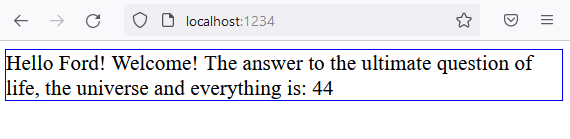
\includegraphics[width=0.8\textwidth]{slike/hello-ford.PNG}
  \caption{Hello World aplikacija, pokrenuta na lokalnom serveru.}
  \label{fig:hello-ford}
\end{figure}

Ukoliko otvorimo ponovo našu aplikaciju u pretraživaču i kliknemo na nju dva puta,
trebalo bi da uоčimo da broj koji se prikazuje na kraju poruke više nije 42, već 44,
dok je pozdravna poruka ovog puta, umesto Arturu, namenjena Fordu (slika \ref{fig:hello-ford})

% U kasnijim poglavljima ćemo se detaljnije upoznati sa time kako ovaj kod zapravo radi.
\section{ Aplikacija "Menadžer Zadataka"}
Pogledaćemo sada malo kompleksniji primer.
U pitanju je aplikacija za upravljanje dnevnim obavezama\footnote{\emph{(eng. TO-DO)} lista.}.
Online verzija ove aplikacije nalazi se na stranici \url{https://pure-framework-todo-demo.netlify.app/}
(Slika \ref{fig:todo-app})

\begin{figure}[!ht]
  \centering
  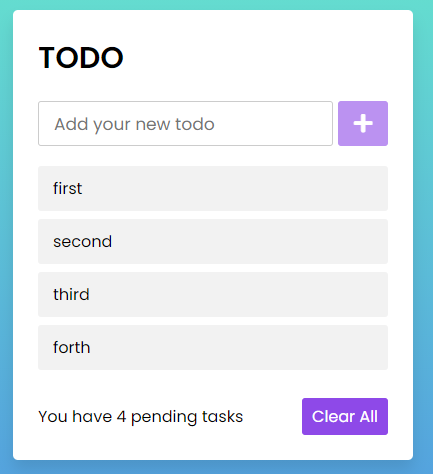
\includegraphics[width=0.5\textwidth]{slike/todo-app-online.PNG}
  \caption{TO DO aplikacija, dostupna online}
  \label{fig:todo-app}
\end{figure}
\pagebreak

\begin{lstlisting}[style=jsStyle, firstnumber=6, caption={Fajl \code{App.ts} nakon dodate funkcionalnosti},label=file:app.ts:2]
import { Component, componentFactory } from "./core";
import { button, div, header, inputText, italic, li, span, ul } from "./htmlElements";
import { ButtonElement } from "./htmlElements/block-elements/buttonElement";

import { store } from "./stores/todo.store";
import { ToDoState } from "./models"

class ToDoListComponent extends Component<ToDoState> {
  template() {
    return div({ class: 'wrapper' }, [
      ...this.headerSegment(),
      this.todoSegment(),
      this.footerSegment(),
    ]);
  }
  ...
}
  \end{lstlisting}

Овај C програм се може превести помоћу преводиоца GCC \cite{gcc}.

% % primer liste
% Можемо правити и набрајања:
% \begin{enumerate}
% \item Анализа 1
% \item Линеарна алгебра
% \item Аналитичка геометрија
% \item Основи програмирања
% \end{enumerate}



% ------------------------------------------------------------------------------
% Literatura
% ------------------------------------------------------------------------------
\literatura

% ==============================================================================
% Završni deo teze i prilozi
\backmatter
% ==============================================================================

% ------------------------------------------------------------------------------
% Biografija kandidata
\begin{biografija}
\textbf{Вук Стефановић Караџић} (\emph{Тршић, 26. октобар/6. новембар
  1787. — Беч, 7. фебруар 1864.}) био је српски филолог, реформатор
српског језика, сакупљач народних умотворина и писац првог речника
српског језика.  Вук је најзначајнија личност српске књижевности прве
половине XIX века. Стекао је и неколико почасних доктората.
Учествовао је у Првом српском устанку као писар и чиновник у
Неготинској крајини, а након слома устанка преселио се у Беч,
1813. године. Ту је упознао Јернеја Копитара, цензора словенских
књига, на чији је подстицај кренуо у прикупљање српских народних
песама, реформу ћирилице и борбу за увођење народног језика у српску
књижевност. Вуковим реформама у српски језик је уведен фонетски
правопис, а српски језик је потиснуо славеносрпски језик који је у то
време био језик образованих људи. Тако се као најважније године Вукове
реформе истичу 1818., 1836., 1839., 1847. и 1852.
\end{biografija}
% ------------------------------------------------------------------------------

\end{document} 